
\section{Results}
\label{mmf-sec:results}
In this section I will present the results when applying MisMatchFinder to various different datasets. First the evaluation of the method on simulated data, which allows accurate and definitive insight into the sensitivity and a proof of concept (\autoref{mmf-sec:simulated data}). Then the analysis of real world applications is displayed in \autoref{mmf-sec:realworld} demonstrating that the method does not only work in cleanly simulated data, but find clinically relevant insight in patient samples.

\subsection{Simulated Data - the validation promised land}
\label{mmf-sec:simulated data}
Just like in \autoref{ch:variantcalling}, the novelty of the approach leads to the issue of no gold standard dataset, with which to evaluate the performance of a new method. While there are low coverage WGS datasets of cancer patients, none of them have validated signatures associated with them. So again simulated data is the optimal starting point to allow both optimisation of parameters as well as granular detection of artefacts which can originate from any step starting from sequencing over mapping to the signature deconvolution. 

\subsubsection{Sequencing errors - there is always a cleaner data}
\label{mmf-sec:cleanSim}
To judge the ability of our approach to filter out sequencing errors, we first simulated ``clean`` sequencing reads with neither germline or somatic variants with the ART simulation suite \cite{Huang2011}. As current estimates of Illumina sequencing is in the range of 1 in 666 to 1 in 1149 \cite{Stoler2021} which is significantly higher than even the highest tumour mutational burdens of  cancers (melanoma: 1 in 5k; tobacco smoking lung cancer: 1 in 100k) it is very important to be able to eliminate as much of the  background noise of sequencing errors as possible.

\begin{figure}[!ht]
\centering
\includegraphics[width=.99\linewidth]{Figures/mismatchrateCleanSequencing.pdf}
\caption[Mismatchrate of different filtering methods]{Mismatchrate of different filtering methods on sequencing data simulated with ART\cite{Huang2011} for both 10x and 3x coverage; Mismatches correspond to simulated sequencing errors; all: no filters, overlap: only use the overlapping parts of paired end reads with consensus building (\protect\autoref{mmf-sec:consensus}), strict OL: overlap but reads \emph{must} agree, high BQ strict OL: strict OL with high BQ in both variants; A) Absolute counts B) counts from A normalised by the number of analysed bases all: all aligned bases, other: number of bases in read overlap}\label{fig:mmf-mismatchrate}
\end{figure}

By only using high base quality mismatches, where both reads agree on the mismatch 99.98\% of all sequencing errors can be eliminated and only 1 in 10M bases will be wrongly counted as a variant (\autoref{fig:mmf-mismatchrate}). This false discovery rate is multiple orders of magnitude lower than before and in a similar range to normal mutationally driven cancers tumour mutational burden \cite{Alexandrov2020,Lawrence2013a}.


\subsubsection{Spike-in signature detection}
\label{mmf-sec:simSingnatures}
With the technical error eliminated in simulated data, the question was would our method work in a real world data, however to establish a baseline for detection limit and sensitivity of the method, we decided to first use a hybrid approach, were we spike-in somatic variants into a genuine low coverage WGS sequencing of a healthy control. That reduces the amount of unknown variability from other published datasets.

While it would be possible simulate the variants completely de novo, without any prior knowledge, we know that somatic mutations follow a certain pattern and there a mutational hotspots \cite{Chen2016,Moore2021}, so we decided to instead use the COSMIC database \cite{Tate2018,WSI2021} as the  to select mutations from. This allows us to select mutations, which definitely occurred in a specific cancer subtype, which leads to a simulation which closer resembles real data. The in-depth protocol is shown in \autoref{ch-mmfAppendix:spikein}. The downside of this method is that the spike-in will not predominantly happen on shorter fragments, as it would be the case with ctDNA. 

In the following section I will discuss the results for the simulation of the very prominent SBS7a signature (see \autoref{fig:sig7a})which is predominantly present in Melanoma (see \autoref{mmf-sec:melaSim}) and secondly the much flatter and more uniform SBS3 (see \autoref{A:fig:sig3}), which is a sign of defective homologous recombination in breast cancers (\autoref{mmf-sec:mbcSim}). 


\begin{figure}[!ht]
\centering
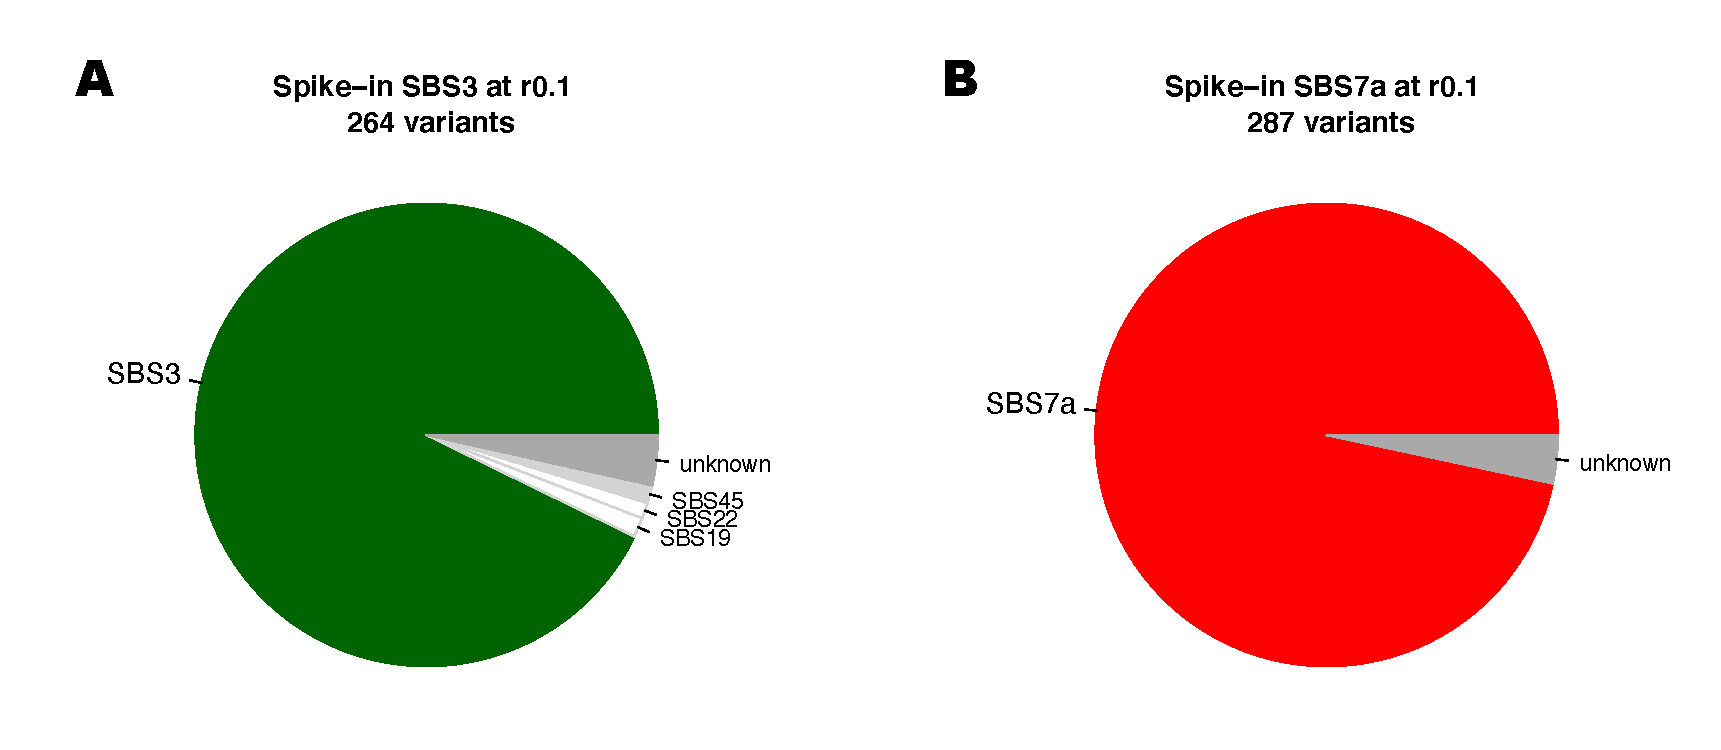
\includegraphics[width=.9\linewidth]{Figures/spikeInSanityCheck.pdf}
\caption[Signature analysis of spike-in somatic variants]{Signature analysis results of spiked-in somatic variants; signatures with a weight less than 1\% were collated into ``unknown``; The original spike-in signature was coloured in green (SBS3) and purple (SBS7a), unrelated signatures are coloured white and signatures corresponding to sequencing artefacts are coloured in lightgrey; r0.1 corresponds to approximately 0.1 variants per mega base; Weights were generated with deconstructSigs \cite{Rosenthal2016} }\label{fig:mmf-spikeinsanity}
\end{figure}

The spike-in was done at multiple different ratios, to simulate varying tumour purity and tumour mutational burden (TMB). \autoref{fig:mmf-spikeinsanity} shows the signature analysis result of the lowest spike-in ratio ``r0.1`` which corresponds to 0.1 somatic variants per mega base and results in approximately 300 variants for the whole genome. As the spike-in process has to satisfy certain quality measures, not all candidate variants can be used. As such, the final simulated BAM contains 264 additional variants for the SBS3 simulation and 287 for the SBS7a equivalent. That corresponds to 304 and 364 ``tumour`` reads respectively within the $\approx$ 261 million reads of the simulated BAM. With increasing ratio, the spike-in signatures show decreasing weights for other signatures, which likely got introduced due to the incomplete spike-in (\autoref{ch-mmfAppendix:spikein}).


\begin{figure}[!ht]
\centering
\includegraphics[width=.99\linewidth]{Figures/deconstructionMethodsDifferences.pdf}
\caption[Signature weight differences for different deconvolution methods]{Signature weight differences for different deconvolution methods; Methods are the quadratic programming (QP) and iterative linea model (ILM); deconvolution was performed on the same counts generated with MisMatchFinder on 7 simulated dataset with increasing mutational burden from 5 to 100 mutations per mega base spike-in; for 0 mutations per mega base, the normal sample used for the spike-in was used}\label{fig:mmf-methodDifferences}
\end{figure}


\paragraph{Melanoma - UV exposure (SBS7a)}
\label{mmf-sec:melaSim}

With melanoma, TMB ranges from 0.1 to 100 mutations per mega base \cite{Alexandrov2020}, however Melanoma is usually seen as a very cancer with very high mutational load, which makes it the ideal target for this new mutational based tool. With only the strict overlap (\autoref{mmf-sec:consensus}) and the germline (\autoref{mmf-sec:germlinefiltering}) filtering enabled, we can see that already from r5, which represents 16899 mutated reads (of 260 Mio.), we see an increase in signature SBS7a. While this signal is likely too low to trust this in a real world setting, with r10, the weight is already 2\% and well established. Secondly, the method is very specific on this dataset, where only SBS7a shows an increase with higher spike-in, which minor leaks to other heavily $C>T$ signatures like SBS2 and SBS30 (\autoref{fig:mmf-methodDifferences},\autoref{fig:mmf-spikeSBS7asignatures}), which partly already stem from the spike-in process, which slightly enriched for SBS2 (\autoref{fig:mmf-spikeinsanity}B ``unknown``). All other signatures, which are present in the normal show a decrease, which is to be expected, as all signature weights need to sum up to one.


\begin{figure}[!ht]
\centering
\includegraphics[width=.99\linewidth]{Figures/SBS7SpikeInSignatureDifferencesFocussed.pdf}
\caption[Signature weights differences from normal for SBS7a spike-in]{Signature weights differences from normal for SBS7a spike-in; Weights were de-constructed with QP method in MisMatchFinder and the weights assigned to the normal sample used for the spike-in were subtracted; Only Signatures with $\text{original weight}\geq 1\%$ or a minimum difference of 0.5\% are shown. The full weights can be seen in \protect\autoref{A:fig:sbs7aspikeindifferences}; r0.1 corresponds to 0.1 mutations per mega base (287 variants) and r100 is the equivalent of 100 mutations per mega base (286974 variants)}\label{fig:mmf-spikeSBS7asignatures}
\end{figure}

\paragraph{BRCA1/2 - Defective homologous recombination-based DNA damage repair (SBS3)}
\label{mmf-sec:mbcSim}

Just as with the SBS7a signatures, even for the much less specific signature SBS3, MisMatchFinder specifically picks out the spike-in signature and does not assign it to any other signature. There is a small increase in SBS4 for the very low mutation rate simulations, where no SBS3 is detected. Not surprisingly, the detection limit for SBS3 is slightly higher than for SBS7a (5 vs. 15 mutations per mega base), because it is a more uniform signal. Exactly as with SBS7a, all other signatures show a slight decrease, to accommodate the additional signature weight which sums to one (\autoref{fig:mmf-methodDifferences}, \autoref{fig:mmf-spikeSBS3signatures}). While this is slightly higher than the currently assumed median TMB in breast cancer, especially triple negative breast cancer (TNBC) has shown a higher TMB, which is at comparable levels to the limit of detection we see in this simulated dataset \cite{BarrosoSousa2020}.

\begin{figure}[!ht]
\centering
\includegraphics[width=.99\linewidth]{Figures/SBS3SpikeInSignatureDifferencesFocussed.pdf}
\caption[Signature weights differences from normal for SBS3 spike-in]{Signature weights differences from normal for SBS3 spike-in; Weights were deconstructed with QP method in MisMatchFinder and the weights assigned to the normal sample used for the spike-in were substracted; Only Signatures with $\text{original weight}\geq 1\%$ or a minimum difference of 0.5\% are shown. The full weights can be seen in \protect\autoref{A:fig:sbs3spikeindifferences}; r0.1 corresponds to 0.1 mutations per megabase (264 variants) and r100 is the equivalent of 100 mutations per megabase (285367 variants)}\label{fig:mmf-spikeSBS3signatures}
\end{figure}

\subsubsection{Germline filtering}
\label{mmf-sec:germlinefiltering}
With real patient data, we can evaluate the effect of removing germline variants from the analysis is. For this I used the same simulated samples from above (\autoref{mmf-sec:simSingnatures}), where the reads are original ctDNA sequencing reads from a healthy person. These reads will have a natural background germline variant signature.

\begin{figure}[!ht]
\centering
\includegraphics[width=.99\linewidth]{Figures/noGermlineFilterAnalysis.pdf}
\caption[Signature analysis without germline variant filtering]{Signature analysis without germline variant filtering; Weights were deconstructed with QP method in MisMatchFinder, but in contrast to \protect\autoref{fig:mmf-methodDifferences}, the filter removing all known germline variants was disabled}\label{fig:mmf-noGermlineFilterAnalysis}
\end{figure}

In stark contrast to the previous analysis (\autoref{fig:mmf-methodDifferences}), when retaining mismatches in known germline variant sites, the sensitivity of the method reduces significantly. Only for the SBS7a spike-in at the very highest mutation frequency (100 mutations per mega base) a signal is detected. This signal is still weaker than what was previously found with just 10 mutations per mega base. Unsurprisingly SBS3 performs worse, just as before, and no signal is detected at all (\autoref{fig:mmf-noGermlineFilterAnalysis}).

This extreme change is caused by the much higher number of mismatches which were used in the analysis ($\approx 1.8$ Mio without germline filter and $\approx 130$K with germline filter).
This increase in mismatches in the analysis dilutes the spike-in variants. \autoref{fig:mmf-percentIncrease} shows that without the germline filter the additional found mismatches never exceeds 5\% which seems to be the detection threshold for SBS7a, as with germline filtering this threshold corresponds nicely with the arise of SBS7a weight in those samples (\autoref{fig:mmf-methodDifferences}).

\begin{figure}[!ht]
\centering
\includegraphics[width=.99\linewidth]{Figures/spikeInPercentage.pdf}
\caption[Percent increase of mismatches in analysis with and without germline filter]{Percent increase of mismatches in analysis with and without germline filter; Values are normalised to the number of mismatches found in the normal sample (depicted as \num{0} mutations per mega base); dotted grey line shows the maximum increase in the left panel (without germline filter)}\label{fig:mmf-percentIncrease}
\end{figure}

While we already know that the spike-in variants were not detected when retaining germline variant sites, the signatures detected in the normal sample are vastly different as well. Without the germline filter, the most prevalent signatures are SBS1 and SBS5 which are thought to be molecular clock like signatures, related to the age of the individual \cite{Alexandrov2020}. In the germline filtered analysis the most prevalent signatures are SBS4 (tabacco smoking), SBS12 (unkown) and SBS46 (sequencing artefact). In general it seems like the germline filter removes predominantly SBS1 and SBS5, while most other signatures remain the same (\autoref{fig:mmf-noGermlinePie}).

As the sample was acquired through a healthy donor blood bank, we have no way to verify if the sample was or is a smoker.

\begin{figure}[!ht]
\centering
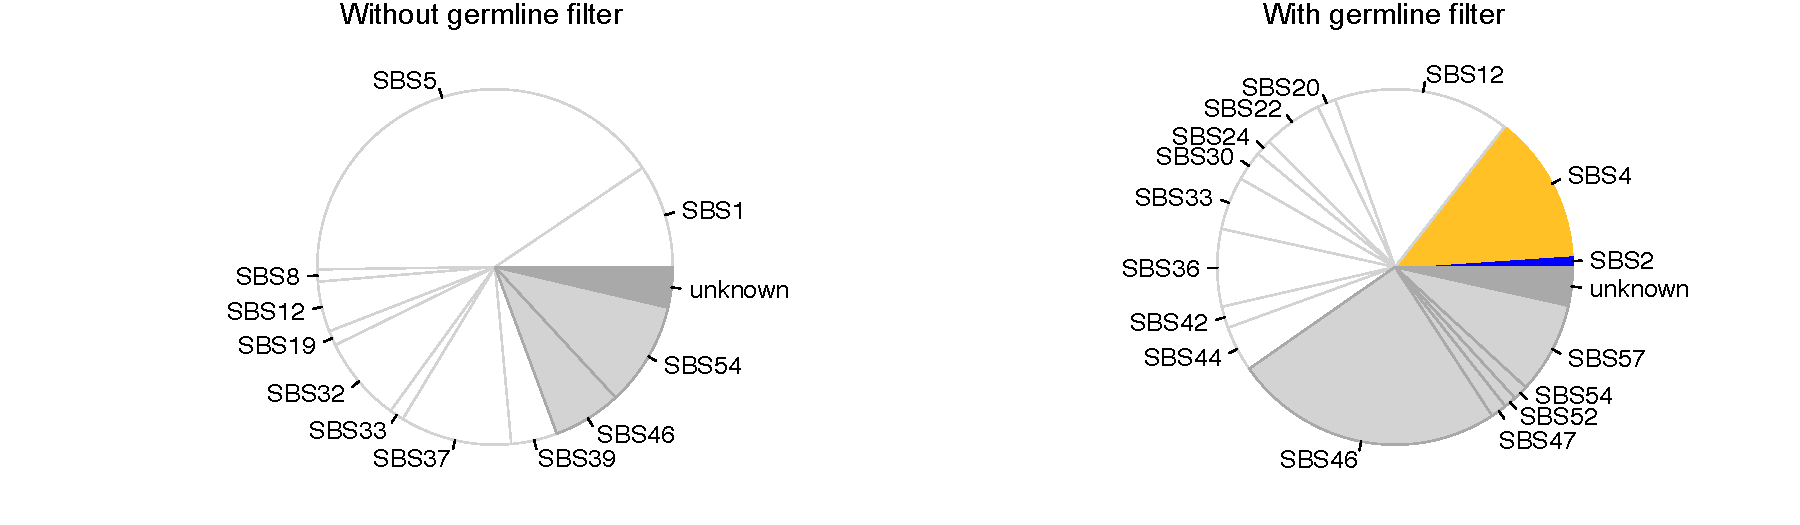
\includegraphics[width=.99\linewidth]{Figures/noGermlineFilterSignaturesPieChart.pdf}
\caption[Signature weights of the normal sample with and without germline filter]{Signature weights of the normal sample with and without germline filter; MisMatchFinder derived signature weights with and without germline filter; weights below 1\% contribution are accumulated in ``unknown`` (darkgrey), lightgrey signatures show sequencing artefact signatures, yellow shows smoking related signatures and blue depicts APOBEC signatures}\label{fig:mmf-noGermlinePie}
\end{figure}
 

This shows that germline filtering similar to the consensus overlap analysis is fundamentally important for the method to recover signal. In the following sections, unless further specified, the germline filter will be enabled for all analysis.





\subsection{Real world data - the only things that matters}
\label{mmf-sec:realworld}

While simulated data is perfect to ensure the method performs as expected in edge cases and to estimate detection limits, only real world data allows the final examination if the model used for analysis can mirror biological concepts. To show our new method is usable for a variety of datasets, we used a mixture of different cancer types from various different sequencers. In \autoref{mmf-sec:healthy} I present the dataset of healthy individuals to show specificity of our method. Then in \autoref{mmf-sec:brcapatients} I present the analysis for metastatic breast cancer patients with matched tumour and germline sequencing. First how efficient germline filtering is in \autoref{mmf-sec:germlineArtifacts} and then how accurate and sensitive our method is when compared to the current gold standard of tumour-normal tissue analysis (\autoref{mmf-sec:matchedMBCB}) and then the envisioned approach of tumour only analysis for clinical samples in \autoref{mmf-sec:tumourOnlyMBCB}.
These analysis were also performed on their melanoma equivalent in \autoref{mmf-sec:matchedMelanoma} for the matched analysis and \autoref{mmf-sec:tumourOnlyMelanoma} to show that the detection is not cancer specific.

\subsubsection{Healthy cohort}
\label{mmf-sec:healthy}

We sequenced the 60 healthy samples, from varying age groups (\num{24}~yrs.-\num{70}~yrs. median: \num{48.5}~yrs.) with 24 males and 36 females, in the exact same way as the tumour only samples for MBCB and melanoma (\autoref{mmf-sec:tumourOnlyMBCB} and \autoref{mmf-sec:tumourOnlyMelanoma} respectively) to an effective average coverage of 8x WGS, with mixed healthy samples and cancer samples on sequencing flow cells to account for batch effects.

\paragraph{Bias detection}
\label{mmf-sec:healthyBias}
This dataset of healthy samples is ideal to detect biases, because any variability that cannot be accounted to either age or gender is unwanted and will affect the cancer samples in the same way. We expect an increased mismatch rate in the older individuals do to the accumulation of somatic mutations, but most of these mutations should be accounted for by SBS1 and SBS5, as they represent the ``clock-like`` signatures \cite{Abascal2021}. Any other signatures would have to be assumed to be either normal variation in the healthy population or technical artefacts.

\todo[inline]{maybe add more info to describe the healthies}


\paragraph{Black list generation}
\label{mmf-sec:healthyBlacklist}
With the strong influence filtering our both technical errors (\autoref{mmf-sec:cleanSim}) and germline variants (\autoref{mmf-sec:germlinefiltering})  as background noise had on our method, we hypothesised that a blacklist of mismatches found in our healthy individuals would help us further cut down on unwanted background signal and refine the somatic mismatch calls. I therefore ran mismatchfinder with significantly relaxed quality cut-offs to capture as much variation as possible. This includes a reduction in mapping quality and base quality as well as not restricting the analysis to the highly accurate overlap part of the paired end reads. However we still restricted the analysis to the same highly mappable areas of the genome the same as for the tumour analysis as well as filtering already known germline variants for a better estimation of the impact of this filter step.

The site files generated through MisMatchFinder were then concatenated and aggregated to multiple blacklists with cut-offs of a variant present in at least 3, 5 or 10 times. The bash code used for the post processing of MisMatchFinder site files can be found in \autoref{lst-mmf:blacklist}.


\begin{lstlisting}[language=bash, caption=Blacklist postprocessing, label={lst-mmf:blacklist}]
awkCounting=$(cat <<'AWK'
{
    key=$1"\t"$2"\t"$3"\t"$4
    counts[key]++
}
END{
    for(i in counts){
        occ = counts[i]
        if(occ >= 3){
            print i"\t"counts[i] > "healthy_blacklist_sites_m3.tsv"
        }
        if(occ >= 5){
            print i"\t"counts[i] > "healthy_blacklist_sites_m5.tsv"
        }
        if(occ >= 10){
            print i"\t"counts[i] > "healthy_blacklist_sites_m10.tsv"
        }
    }
}
AWK
)

cat *_sites.tsv | awk "$awkCounting"
\end{lstlisting}




\todo[inline]{Add the health cohort in there/ possible age}

\subsubsection{MBCB patient samples}
\label{mmf-sec:brcapatients}
The first dataset of patients is two previously published BRCA1/2 positive breast cancers\todo{are they actually published?}. The data contains matched tumour, germline and ctDNA sequencing as high depth WGS for both patients. With the matched normal, we can use the current standard protocol of somatic mutational pattern analysis (\autoref{mmf-sec:signatureanalysis}) and compare it with our new method (\autoref{mmf-sec:matchedMBCB}). 

As the sequencing data of the ctDNA is much higher depth than what is used in standard clinical practice, we down sample the data to 10x coverage, which is also the coverage of the simulated data. By using numerous different seeds for the sampling, we can generate pseudo technical replicates of the sequencing (\autoref{ch-mmfAppendix:subsampling}), which then in term can give an approximation of the stability of the results for both the tissue and the ctDNA samples .

And secondly we analysed a set of tumour only sequencing samples, how they would be available in clinical testing, e.g. copy number analysis \cite{Homburger2019,Chen2021}. To show that our method can be applied to supply additional clinically relevant information from already available data (\autoref{mmf-sec:tumourOnlyMBCB}). 

\todo[inline]{add the subsampled data}

\paragraph{Germline artifacts}
\label{mmf-sec:germlineArtifacts}
As I have pointed out above, how important the germline filter step is to boost the signal of somatic variants (\autoref{mmf-sec:germline}), we were interested how many germline variants were not filtered out with our method. The high depth matched healthy WGS samples of the breast cancer dataset is ideal for this analysis. I called germline variants on the matched normal using Strelka2 and compared the called variants with the sites which MisMatchFinder found to be somatic (retained after germline filtering) on the sub-sampled data.  All variants with any quality filter assigned by Strelka2 were considered for this analysis, such that possible clonal hematopoiesis (CH) variants are still considered. \autoref{tab:mmf-germlineArtifacts} shows that on average 2100 germline variants are not filtered out. However, this only equates to 0.9\% for MBCB196 and 1.5\% for MBCB298 of all sites found to be mutated. The exact numbers depend on the strictness of the parameters of the analysis as well as the mutation rate of the sample, so they should only be taken as a guideline.

Nevertheless, this result combined with the effective filtering of technical errors (\autoref{mmf-sec:cleanSim}) suggests, that the remaining sites are somatic mutations of either the healthy tissue or the cancer.

\begin{table}
\caption[Germline variants retained after germline filtering]{Germline variants retained after germline filtering with in MisMatchFinder analysis; Default parameters were used when running MisMatchFinder with gnomAD zarr for filtering. seed column shows the seed used to subsample the high depth sequencing BAM, ``mismatch sites`` column contains number of sites found to be changed, ``germline sites`` contains the number of sites also found with germline variant calling, fraction shows fraction of column 4 and 3}\label{tab:mmf-germlineArtifacts}
\centering
\begin{tabular}{c|c|c|c|c}
\toprule
\textbf{Patient ID} & \textbf{seed} & \textbf{mismatch sites} & \textbf{germline sites} & \textbf{fraction} \\
\midrule
 & \num{1007} & \num{216950} &  \num{2107} & \num{0.0097}\\ 
 & \num{1234} & \num{217145} &  \num{2073} & \num{0.0095}\\ 
 & \num{1337} & \num{216823} &  \num{2080} & \num{0.0096}\\ 
 & \num{1717} & \num{217593} &  \num{2089} & \num{0.0096}\\ 
 & \num{2358} & \num{217317} &  \num{2097} & \num{0.0096}\\ 
 & \num{3311} & \num{217219} &  \num{2046} & \num{0.0094}\\ 
 & \num{5229} & \num{216876} &  \num{2062} & \num{0.0095}\\ 
 & \num{6060} & \num{217388} &  \num{2080} & \num{0.0096}\\ 
\multirow{-9}{*}{MBCB196} & \num{9876} & \num{217656} &  \num{2008} & \num{0.0092}\\ 
\midrule
 & \num{1756} & \num{148495} &  \num{2168} & \num{0.0146}\\ 
 & \num{3599} & \num{149901} &  \num{2224} & \num{0.0148}\\ 
 & \num{4117} & \num{149382} &  \num{2277} & \num{0.0152}\\ 
 & \num{4306} & \num{149549} &  \num{2248} & \num{0.0150}\\ 
 & \num{4359} & \num{149805} &  \num{2205} & \num{0.0147}\\ 
 & \num{5788} & \num{150103} &  \num{2241} & \num{0.0149}\\ 
 & \num{5887} & \num{150099} &  \num{2287} & \num{0.0152}\\ 
 & \num{8387} & \num{149533} &  \num{2248} & \num{0.0150}\\ 
\multirow{-9}{*}{MBCB298} & \num{9754} & \num{149547} &  \num{2229} & \num{0.0149}\\
\bottomrule
\end{tabular}
\end{table}


\paragraph{Matched WGS samples - when you know what the results should be}
\label{mmf-sec:matchedMBCB}

\begin{figure}[!ht]
\centering
\includegraphics[width=.99\linewidth]{Figures/mbcbWESsignatures.pdf}
\caption[Signature weights for the WGS of two MBCB patients]{Signature weights for the WGS of two MBCB patients; Colours show cancer associated signatures: blue (APOBEC), red (UV exposure), orange (tobacco), purple (chemotherapy), light grey (sequencing artefacts), dark grey (everything below 1\% weight)}\label{fig:mmf-mbcbWGSsigPie}
\end{figure}
 

\paragraph{Tumour only WGS samples - the large scale clinical approach}
\label{mmf-sec:tumourOnlyMBCB}

\subsubsection{Melanoma patients}
\label{mmf-sec:melpatients}

For melanoma real world data, we analysed multiple datasets, which allowed to highlight and dissect specific aspects of signature detection from lcWGS when dealing with melanoma. First I will show the results on a set of two patients, were WES of tumour tissue, normal tissue and both cfDNA samples is available on top of lcWGS of the cfDNA (\autoref{mmf-sec:matchedMelanoma}) and then I will highlight the results of the analysis of a bigger dataset of melanoma patients without matched normals but with varying tumour fraction (\autoref{mmf-sec:tumourOnlyMelanoma}).


\paragraph{Matched WES samples - when you know what the results should be}
\label{mmf-sec:matchedMelanoma}
With the help of the WES of both the tissue and the cfDNA samples, we know what the expected outcome for each of the lcWGS samples is, as the standard procedure for signature detection starts with somatic variants.  Strelka2 was used to call somatic variants and the high confidence somatic SNPs were then used in R to generate signature weights with deconstructSigs. As the most recent signatures were generated using whole genome sequencing, the input was normalised with the \lq \emph{exome2genome}\rq~option when calculating weights.


\begin{figure}[!ht]
\centering
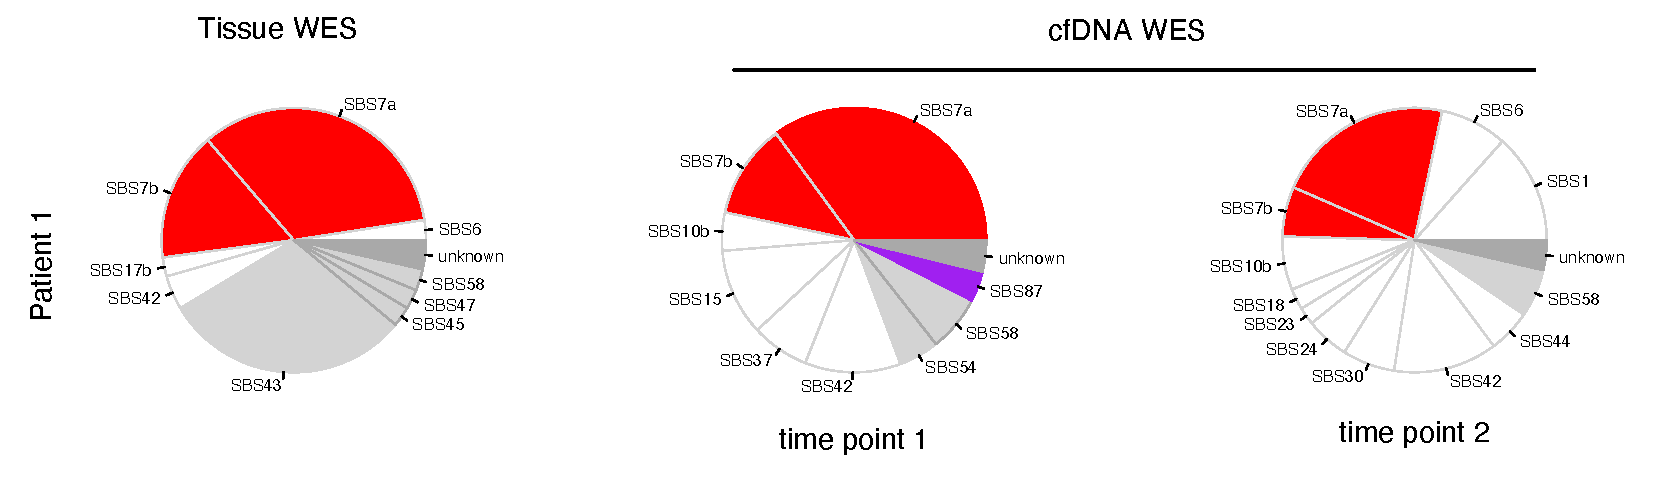
\includegraphics[width=.99\linewidth]{Figures/melanomaWESsignatures.pdf}
\caption[Signature weights for the WES of two melanoma patients]{Signature weights for the WES of two melanoma patients; First column shows the results for the tissue baseline and middle and right column show the cfDNA; Colours show cancer associated signatures: blue (APOBEC), red (UV exposure), orange (tobacco), purple (chemotherapy), light grey (sequencing artefacts), dark grey (everything below 1\% weight)}\label{fig:mmf-melaWESsigPie}
\end{figure}
 
For Patient 1, both the tissue as well as the cfDNA samples show a very high signature weight related to UV radiation SBS7a and SBS7b ($ \text{combined}\geq 30\%$ however patient 2 only shows very little SBS7a in only the cfDNA samples. 

\paragraph{Large detection level cohort - how sensitive can we be?}
\label{mmf-sec:tumourOnlyMelanoma}


\subsection{Summary}
\todo[inline]{Dont know if we need this}
